\documentclass{ximera}

\graphicspath{  %% When looking for images,
{./}            %% look here first,
{./pictures/}   %% then look for a pictures folder,
{../pictures/}  %% which may be a directory up.
{../../pictures/}  %% which may be a directory up.
{../../../pictures/}  %% which may be a directory up.
{../../../../pictures/}  %% which may be a directory up.
}

\usepackage{listings}
\usepackage{circuitikz}
\usepackage{xcolor}
\usepackage{amsmath,amsthm}
\usepackage{subcaption}
\usepackage{graphicx}
\usepackage{tikz}
\usepackage{tikz-3dplot}
\usepackage{amsfonts}
\usepackage{mdframed} % For framing content
\usepackage{tikz-cd}

  \renewcommand{\vector}[1]{\left\langle #1\right\rangle}
  \newcommand{\arrowvec}[1]{{\overset{\rightharpoonup}{#1}}}
  \newcommand{\ro}{\texttt{R}}%% row operation
  \newcommand{\dotp}{\bullet}%% dot product
  \renewcommand{\l}{\ell}
  \let\defaultAnswerFormat\answerFormatBoxed
  \usetikzlibrary{calc,bending}
  \tikzset{>=stealth}
  




%make a maroon color
\definecolor{maroon}{RGB}{128,0,0}
%make a dark blue color
\definecolor{darkblue}{RGB}{0,0,139}
%define the color fourier0 to be the maroon color
\definecolor{fourier0}{RGB}{128,0,0}
%define the color fourier1 to be the dark blue color
\definecolor{fourier1}{RGB}{0,0,139}
%define the color fourier 1t to be the light blue color
\definecolor{fourier1t}{RGB}{173,216,230}
%define the color fourier2 to be the dark green color
\definecolor{fourier2}{RGB}{0,100,0}
%define teh color fourier2t to be the light green color
\definecolor{fourier2t}{RGB}{144,238,144}
%define the color fourier3 to be the dark purple color
\definecolor{fourier3}{RGB}{128,0,128}
%define the color fourier3t to be the light purple color
\definecolor{fourier3t}{RGB}{221,160,221}
%define the color fourier0t to be the red color
\definecolor{fourier0t}{RGB}{255,0,0}
%define the color fourier4 to be the orange color
\definecolor{fourier4}{RGB}{255,165,0}
%define the color fourier4t to be the darker orange color
\definecolor{fourier4t}{RGB}{255,215,0}
%define the color fourier5 to be the yellow color
\definecolor{fourier5}{RGB}{255,255,0}
%define the color fourier5t to be the darker yellow color
\definecolor{fourier5t}{RGB}{255,255,100}
%define the color fourier6 to be the green color
\definecolor{fourier6}{RGB}{0,128,0}
%define the color fourier6t to be the darker green color
\definecolor{fourier6t}{RGB}{0,255,0}

%New commands for this doc for errors in copying
\newcommand{\eigenvar}{\lambda}
%\newcommand{\vect}[1]{\mathbf{#1}}
\renewcommand{\th}{^{\text{th}}}
\newcommand{\st}{^{\text{st}}}
\newcommand{\nd}{^{\text{nd}}}
\newcommand{\rd}{^{\text{rd}}}
\newcommand{\paren}[1]{\left(#1\right)}
\newcommand{\abs}[1]{\left|#1\right|}
\newcommand{\R}{\mathbb{R}}
\newcommand{\C}{\mathbb{C}}
\newcommand{\Hilb}{\mathbb{H}}
\newcommand{\qq}[1]{\text{#1}}
\newcommand{\Z}{\mathbb{Z}}
\newcommand{\N}{\mathbb{N}}
\newcommand{\q}[1]{\text{``#1''}}
%\newcommand{\mat}[1]{\begin{bmatrix}#1\end{bmatrix}}
\newcommand{\rref}{\text{reduced row echelon form}}
\newcommand{\ef}{\text{echelon form}}
\newcommand{\ohm}{\Omega}
\newcommand{\volt}{\text{V}}
\newcommand{\amp}{\text{A}}
\newcommand{\Seq}{\textbf{Seq}}
\newcommand{\Poly}{\textbf{P}}
\renewcommand{\quad}{\text{    }}
\newcommand{\roweq}{\simeq}
\newcommand{\rowop}{\simeq}
\newcommand{\rowswap}{\leftrightarrow}
\newcommand{\Mat}{\textbf{M}}
\newcommand{\Func}{\textbf{Func}}
\newcommand{\Hw}{\textbf{Hamming weight}}
\newcommand{\Hd}{\textbf{Hamming distance}}
\newcommand{\rank}{\text{rank}}
\newcommand{\longvect}[1]{\overrightarrow{#1}}
% Define the circled command
\newcommand{\circled}[1]{%
  \tikz[baseline=(char.base)]{
    \node[shape=circle,draw,inner sep=2pt,red,fill=red!20,text=black] (char) {#1};}%
}

% Define custom command \strikeh that just puts red text on the 2nd argument
\newcommand{\strikeh}[2]{\textcolor{red}{#2}}

% Define custom command \strikev that just puts red text on the 2nd argument
\newcommand{\strikev}[2]{\textcolor{red}{#2}}

%more new commands for this doc for errors in copying
\newcommand{\SI}{\text{SI}}
\newcommand{\kg}{\text{kg}}
\newcommand{\m}{\text{m}}
\newcommand{\s}{\text{s}}
\newcommand{\norm}[1]{\left\|#1\right\|}
\newcommand{\col}{\text{col}}
\newcommand{\sspan}{\text{span}}
\newcommand{\proj}{\text{proj}}
\newcommand{\set}[1]{\left\{#1\right\}}
\newcommand{\degC}{^\circ\text{C}}
\newcommand{\centroid}[1]{\overline{#1}}
\newcommand{\dotprod}{\boldsymbol{\cdot}}
%\newcommand{\coord}[1]{\begin{bmatrix}#1\end{bmatrix}}
\newcommand{\iprod}[1]{\langle #1 \rangle}
\newcommand{\adjoint}{^{*}}
\newcommand{\conjugate}[1]{\overline{#1}}
\newcommand{\eigenvarA}{\lambda}
\newcommand{\eigenvarB}{\mu}
\newcommand{\orth}{\perp}
\newcommand{\bigbracket}[1]{\left[#1\right]}
\newcommand{\textiff}{\text{ if and only if }}
\newcommand{\adj}{\text{adj}}
\newcommand{\ijth}{\emph{ij}^\text{th}}
\newcommand{\minor}[2]{M_{#2}}
\newcommand{\cofactor}{\text{C}}
\newcommand{\shift}{\textbf{shift}}
\newcommand{\startmat}[1]{
  \left[\begin{array}{#1}
}
\newcommand{\stopmat}{\end{array}\right]}
%a command to give a name to explorations and hints and theorems
\newcommand{\name}[1]{\begin{centering}\textbf{#1}\end{centering}}
\newcommand{\vect}[1]{\vec{#1}}
\newcommand{\dfn}[1]{\textbf{#1}}
\newcommand{\transpose}{\mathsf{T}}
\newcommand{\mtlb}[2][black]{\texttt{\textcolor{#1}{#2}}}
\newcommand{\RR}{\mathbb{R}} % Real numbers
\newcommand{\id}{\text{id}}

\author{Zack Reed}
%%Snapp, B. (2024). Ximera la-carte: An open-source platform for interactive textbooks. https://ximera.osu.edu
%%OpenAI. (2023). ChatGPT (Mar 14 version) [Large language model]. https://chat.openai.com/chat

\title{Learning Activity: Vectors in the Physical World}

\begin{document}
\begin{abstract}
    An introduction to how vectors provide a lens for understanding the world around us.
\end{abstract}
\maketitle

\section*{Vectors in the Physical World}

If you're coming from STEM, you've probably more accustomed to thinking about vectors in relation to physical quantities like speed, acceleration, force, and electric fields. Whereas in other settings (such as the apple example above), the vector representations can be somewhat abstract, or arbitrary, and the structure of the geometry is key, in the physical world the geometry of vectors themselves are much more closely linked to a physical interpretation.

\section*{A Physical Example: Velocity}

Velocity, acceleration, and forces naturally lend themselves to vector representation, and point us towards other properties of vectors that we care to measure, namely those of \textit{magnitude} and \textit{direction}. This example will emphasize the utility of \textit{addition} and \textit{scaling} as fundamental to vectors.

\begin{example}
    
  Suppose an airplane is flying from Daytona Beach to a location roughly northeast of Daytona Beach at a speed of $300$ knots. If we were in a scalar context, $300$ would be the only necessary speed information, as we could distinguish $300$ from $-300$ as being "forward" or "backward" motion, and the value $300$ to give the speed. In the spatial world, however, objects move in directions, and so we need to know the direction of the airplane's velocity as well.

  In the following GeoGebra application, scaled down so that $300$ knots has a value of $3$, the airplane's destination is located at around $(11.14,4.46)$, and the airplane's starting location is at $(0,0)$. 

  \begin{center}
    \geogebra{qytw4pbt}{801}{575}
  \end{center}

  The vector $\vec{D}=[11.14,4.46]$ gives the airplane a direction, but we also need to factor in the ariplane's speed. We want the geometric length of the vector to be the plane's speed ($300$ knots), so we want the plane's velocity vector to be an arrow in the direction of $\vec{D}$, but only a length $3$. The vector length is called its \textit{magnitude}, and for our purposes its magnitude directly correlates to speed. As such, we need a way to geometrically determine the lengths of vectors, for which we'll use the Pythagorean theorem.

  \begin{remark}

    Distance and length are two sides of the same coin for standard Euclidean space, and the Pythagorean theorem key.

    Consider two points $P=(p_1,p_2)$ and
    $Q=(q_1,q_2)$ in the plane, as in the following picture.
   
      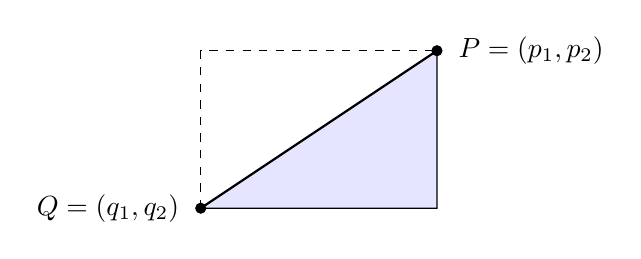
\begin{tikzpicture}[scale=1]
        \draw[dashed] (0,0) -- (0,2) -- (3,2);
        \draw[fill=blue!10] (0,0) -- (3,0) -- (3,2) -- cycle;
        \draw[thick] (0,0) -- (3,2);
        \draw[fill](0,0) circle [radius=1.8pt] node[left=1ex]{$Q=(q_1,q_2)$};
        \draw[fill](3,2) circle [radius=1.8pt] node[right=1ex]{$P=(p_1,p_2)$};
      \end{tikzpicture}

    The distance between $P$ and $Q$ is shown in the picture as a solid
    line, which is the hypotenuse of a right triangle.  The lengths of the
    two other sides of this triangle are $(p_1-q_1)$ and
    $(p_2-q_2)$. Therefore, the Pythagorean Theorem implies the
    length of the hypotenuse (and thus the distance between $P$ and $Q$)
    equals
    \begin{equation*}
      d(P,Q)
      =\sqrt{(p_1-q_1)^2+(p_2-q_2)^2}.
    \end{equation*}

    Similarly in 3 dimensions, points $P=(p_1,p_2,p_3)$ and
    $Q = (q_1,q_2,q_3)$ have a distance of $d(P,Q)=\sqrt{(p_1-q_1)^2+(p_2-q_2)^2+(p_3-q_3)^2}$.

      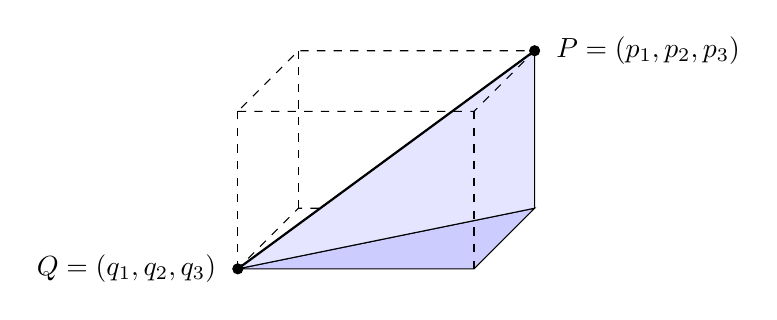
\begin{tikzpicture}[scale=1]
        \draw[dashed] (3,0,-2) -- (0,0,-2) -- (0,0,0);
        \draw[dashed] (0,0,0) -- (0,2,0);
        \draw[dashed] (0,0,-2) -- (0,2,-2);
        \draw[fill=blue!20] (0,0,0) -- (3,0,0) -- (3,0,-2) -- cycle;
        \draw[fill=blue!10] (0,0,0) -- (3,0,-2) -- (3,2,-2) -- cycle;
        \draw[dashed] (0,2,0) -- (3,2,0) -- (3,2,-2) -- (0,2,-2) -- cycle;
        \draw[dashed] (3,0,0) -- (3,2,0);
        \draw[thick] (0,0,0) -- (3,2,-2);
        \draw[fill](0,0,0) circle [radius=1.8pt] node[left=1ex]{$Q=(q_1,q_2,q_3)$};
        \draw[fill](3,2,-2) circle [radius=1.8pt] node[right=1ex]{$P=(p_1,p_2,p_3)$};
        %\draw[fill](3,0,-2) circle [radius=1.8pt] node[right=1ex]{$R=(p_1,p_2,q_3)$};
        %\draw[fill](3,0,0) circle [radius=1.8pt] node[right=1ex]{$S=(p_1,q_2,q_3)$};
      \end{tikzpicture}

  
\begin{definition}\name{Distance between points}
  
      Let $P=(p_1,\ldots,p_n)$ and $Q=(q_1,\ldots,q_n)$ be two points in
      $\R^n$. Then the \textbf{distance}%
      \index{distance!point to point} between these points is defined as
      \begin{equation*}
        d(P, Q) = \sqrt{(p_1-q_1)^2 + \ldots + (p_n-q_n)^2}.
      \end{equation*}
      This formula is also called the \textbf{distance formula}%
      \index{distance formula}. We may also write $\left\|PQ\right\|$ for the
      distance between $P$ and $Q$.
    \end{definition}

A vector's \textit{magnitude}, then, can be thought of as its distance from $\vec{0}$. 

\begin{definition}\name{Length of a vector}
  Let
  \begin{equation*}
    \vec{u} = \startmat{c} u_1 \\ \vdots \\ u_n \stopmat
  \end{equation*}
  be a vector in $\R^n$. Then the \textbf{length}%
  \index{vector!length}%
  \index{length of a vector} of $\vec{u}$, written $\left\| \vec{u} \right\|$,
  is given by
  \begin{equation*}
    \left\| \vec{u} \right\| = \sqrt{u_1^2 + \ldots + u_n^2}.
  \end{equation*}
  The length of a vector is also sometimes called its
  \textbf{magnitude}%
  \index{magnitude!of a vector}%
  \index{vector!magnitude} or its
  \textbf{norm}%
  \index{norm!in Rn@in $\R^n$}%
  \index{vector!norm}.
\end{definition}

  \end{remark}

  So, to describe our plane's velocity vector, it needs to be in the same direction as the vector $\vec{D}=[11.14,4.46]$, but with a length of $3$. Using the definition above, the length of the destination vector is $\left\|\vec{D}\right\|=\sqrt{11.14^2+4.46^2}\approx 12$. To get a vector of length $3$, to re-size its coordinates to match the right scale, so we divide each coordinate by $\left\|\vec{D}\right\|$ and multiply by $3$, yielding the vector $$\vec{v}=\left[11.14\cdot \frac{3}{12},4.46\cdot \frac{3}{12}\right]\approx \left[\frac{11.14}{4},\frac{4.46}{4}\right] = [2.79,1.12].$$

  Note that to re-size $\vec{v}$ so that it has a length of $3$, we also determined the amount by which we scaled the destination vector $\vec{D}$ to get $\vec{v}$. Knowing that each coordinate of $\vec{v}$ is $\frac{1}{4}$ of the corresponding coordinate of $\vec{D}$ (say, in ``knots-per-hour''), the plane will reach the destination in $\answer{4}$ hours.

  Hence, the geometric vector in the applet represents the plane's speed and direction. This is an example of \emph{scalar multiplication} of a vector, where we multiply each coordinate of the vector by a scalar.

  \begin{remark}

    This leads to a definition.

    \begin{definition}\name{Scalar Multiplication of a Vector}

      Let $\vec{v} = \startmat{c} v_1 \\ \vdots \\ v_n \stopmat$ be a vector in $\R^n$ and let $c$ be a scalar. The \textbf{scalar multiple} of $\vec{v}$ by $c$ is the vector
      \begin{equation*}
        c\vec{v} = \startmat{c} cv_1 \\ \vdots \\ cv_n \stopmat.
      \end{equation*}

    \end{definition}

    In other words, we multiply a vector by a scalar by multiplying each of its coordinates by the scalar. The vector represents velocity because the scale is with respect to time, so each coordinate gives how far in the coordinate directions the plane will travel in one hour.

  \end{remark}


\end{example}

\section*{Blowing Off Course}
  
  Suppose that for the entire trip, the wind is blowing exactly in the northwestern direction at a speed of $100*\sqrt(2)$ knots ($\sqrt{2}$ in the applet). The wind (uniformly applied throughout the trip) is imposing another velocity on the plane. To determine the plane's new trajectory, we need the notion of \textit{vector addition}.



  The plane's velocity vector is given in the GeoGebra environment below. You can always see its intended trajectory (and original velocity vector) in purple. Hit the ``Animate'' button to see the plane's path.

  A northwestern wind moves equally to the right as it does upward, so with a speed of $\sqrt{2}$ the wind vector is $\vec{w}=[\answer{1},\answer{1}]$.

  \begin{solution}

    You can use $[a,a]$ for the direction vector moving equally westward and northward, and then keeping the pythagorean theorem in mind, $\sqrt{2}=\sqrt{1^2+1^2}$, you can determine the wind vector $\vec{w}=[1,1]$.

  \end{solution}

  Select the "Allow Wind" checkbox and enter $\vec{w}$ as the wind vector, and then hit "Set Wind". This will visualize a new trajectory for the plane. The black vector is the plane's new velocity vector, the purple vector is the plane's original velocity vector, and the blue vector is the wind vector. Note that to get the black vector, you first move along the purple vector, and then move along the blue vector starting at the head of the purple vector.

  Since the plane maintains the velocity vectors throughout the flight, you can see the plane's final destination by hitting the "Animate" button, noting that the velocity is constantly affecting the distance traveled.
  \begin{center}
    \geogebra{qytw4pbt}{801}{575}
  \end{center}


This is how we geometrically interpret \emph{vector addition}. If $\vec{v}$ is the plane's velocity vector, and $\vec{w}$ is the wind vector, then the plane's new velocity vector is $\vec{v}+\vec{w}$. 

Numerically, you find this by adding the coordinates of the vectors. So, if $\vec{v}=[2.79,1.12]$ and $\vec{w}=[1,1]$, then 

\[
\vec{v}+\vec{w}=[2.79+1,1.12+1]=[\answer{3.79},\answer{2.12}].
\]

\begin{definition}\name{Addition of vectors in $\R^n$}
  For vectors $\vec{u}=\startmat{c}
    u_1 \\
    \vdots \\
    u_n
  \stopmat,\; \vec{v}= \startmat{c}
    v_1 \\
    \vdots \\
    v_n
  \stopmat$ in $\R^n$, the sum $\vec{u}+\vec{v}$ in $\R^n$ is defined
  by
  \begin{equation*}
    \vec{u}+\vec{v} = \startmat{c}
      u_1 \\
      \vdots \\
      u_n
    \stopmat +  \startmat{c}
      v_1 \\
      \vdots \\
      v_n
    \stopmat
    = \startmat{c}
      u_1+v_1 \\
      \vdots \\
      u_n+v_n
    \stopmat.
  \end{equation*}
\end{definition}

The geometry and the numerical interpretations together make sense, since you can imagine getting to the tip of the sum vector by 


\begin{tikzpicture}

  % Draw x and y axes
  \draw[->] (-1,0) -- (6,0); %node[right] {$x$};
  \draw[->] (0,-1) -- (0,6); %node[above] {$y$};
  
  % Define the origin
  \coordinate (O) at (0,0);
  
  % Define vectors u and v
  \coordinate (U) at (3,1);   % Vector u components (3, 2)
  \coordinate (V) at (1,3);   % Vector v components (2, 1)
  
  % Calculate u + v
  \coordinate (UV) at ($(U)+(V)$);
  
  % Draw vector u
  \draw[->, thick, red] (O) -- (U) node[midway, above] {$\vec{u}$};
  
  % Draw vector v starting from tip of u
  \draw[->, thick, red] (U) -- (UV) node[midway, right] {$\vec{v}$};
  
  % Draw resultant vector u + v
  \draw[->, thick, blue] (O) -- (UV) node[midway, above left] {$\vec{u} + \vec{v}$};
  
  % Draw dashed lines to form right triangles for u
  \draw[dashed] (U) -- (U |- O) -- (O);
  
  % Draw dashed lines to form right triangles for v
  \draw[dashed] (UV) -- (UV |- U) -- (U);
  
  % Draw dashed lines to form right triangles for u + v
  %\draw[dashed] (UV) -- (UV |- O) -- (O);
  
  % Mark right angles
  % For vector u
  \draw ($(U) + (-0.2,0)$) -- ++(0,-0.2) -- ++(0.2,0);
  % For vector v
  \draw ($(UV) + (-0.2,0)$) -- ++(0,-0.2) -- ++(0.2,0);
  
\end{tikzpicture}

You can move horizontally below (or above) the first coordinate of $u+v$ by moving $u_1$ then $v_1$ (hence, $u_1+v_1$), and similarly for the second coordinate. This is the geometric interpretation of vector addition.



\section*{Course Correction}

  By how much do you need to correct the plane to reach its destination in a straight shot? There are two immediately avaialable options, with one making more practical sense than the other. 

\begin{problem}
  First, you can direct the plane against the wind, so that the wind velocity is canceled out and the plane can return to its original course. This adds the negative of $\vec{w}$ to $\vec{v}$, so that the plane's new velocity vector is $\vec{v}+\vec{w}-\vec{w}=\vec{v}$.

  Try this in the applet, by selecting the "Allow Correction" check box and entering $-\vec{w}=[-1,-1]$. Setting the wind and correction then shows the plan on its original course, with the velocity vectors first moving along the initial velocity, then along the wind, then back down reversing the velocity. 

  \begin{center}
    \geogebra{qytw4pbt}{801}{575}
  \end{center}

  You could take a more efficient route, however, by noting that the wind does push the plane further north and west than it would have gone otherwise, so there is some added speed in a direction similar to the intended direction. If you set the correction vector correctly, you re-orient the plane along its intended path but also with less travel time than the original path.

  First, do so in the applet, then solve for the correction vector $\vec{c}$ algebraically below.
  
  We want $\vec{v}+\vec{w}+\vec{c}$ to be in the same direction as $\vec{v}$, but with a magnitude greater than $3$. Assuming that we want to minimally increase the plane's engine use, let's just give the correction vector a vertical component (really we would want to go at a right angle to the wind vector, but we'll cover that later). 

  So, we want $\vec{v}+\vec{w}+\vec{c}=[2.79+1,1.12+1+c_2]=[3.79,2.12+c_2]$ to be in the same direction as $\vec{v}=[2.79,1.12]$. This is hard to do unless we have a common scale, so we need to think \emph{just} about direction for a moment, rather than direction and length together. This is the notion of \textit{unit vectors} (or \textit{direction vectors}).

  \begin{definition}\name{Unit Vectors}

    A \textbf{unit vector} is a vector of length $1$. 

    In $\R^n$, the standard coordinate vectors are examples of unit vectors. In $\R^3$, the coordiante vectors are $\vect{i}=[1,0,0]$, $\vect{j}=[0,1,0]$, and $\vect{k}=[0,0,1]$.
  \end{definition}

  Since we want $\vec{v}+\vec{w}+\vec{c}$ and $\vec{v}$ to be in the same direction, we can solve for the coordiantes of $\vec{v}+\vec{w}+\vec{c}$ in the following way: 

\begin{enumerate}

\item Find the unit vector $\vec{u}$ in the direction of $\vec{v}$. Since $\vec{v}$ is fixed, we can find $\vec{u}$ by dividing $\vec{v}$ by its length.
\item Since $\vec{v}+\vec{w}+\vec{c}$ is in the same direction as $\vec{v}$, which is in the same direction as $\vec{u}$, all three vectors are scalar multiples of each other. Geometrically, each vector is a stretched or compressed version of the others. So we can solve for the scalar $s$ such that $\vec{v}+\vec{w}+\vec{c}=s\vec{u}$.
\item The vector equation $\vec{v}+\vec{w}+\vec{c}=s\vec{u}$ gives us two scalar linear equations, which we can solve for the two unknowns $s$ and $c_2$.

\begin{hint}

  We'll develop more sophisticated ways of doing this in Chapter 3, but for now you solve a system of two scalar linear equations by first isolating one variable, substituting it into the other equation, and solving for the other variable to then substitute back.

  For instance, the steps to solving 

  \[
  \begin{array}{ccc}
    2x+y&=&3\\
    x-2y&=&-1
  \end{array}
  \]

  would be to first isolate $x$ in the second equation, so that $x=2y+1$, then substitute this into the first equation to get $2(2y+1)+y=3$, which simplifies to $5y+2=3$, so $y=1/5$. Substituting this back into $x=2y+1$ gives $x=7/5$.

\end{hint}

\end{enumerate}

  \begin{solution}

  $\left\|\vec{v}\right\|=\sqrt{2.79^2+1.12^2}\approx 3$, so $\vec{u}=\left[\frac{2.79}{3},\frac{1.12}{3}\right]\approx [0.93,0.37]$. 

  The vector equation $\vec{v}+\vec{w}+\vec{c}=s\vec{u}$ can be stated in components as $s[.93,.37]=[3.79,2.12+c_2]$. This gives us two equations

  \begin{align*}
    .93s&=3.79\\
    .37s&=2.12+c_2
  \end{align*}

  The first equation gives $s\approx 4.08$, and substituting this into the second equation gives $c_2\approx .37s-2.12=.37(4.08)-2.12\approx -.61$. So, the correction vector is $\vec{c}=[0,-.61]$.

  \end{solution}

  When all is said and done, the plane's new velocity vector is $\vec{v}+\vec{w}+\vec{c}=[2.79, 1.12]+[1,1]+[0,\answer{-.61}]\approx [3.79,\answer{1.51}]$. With this velocity, the plane will travel along the same path but get to the destination in less time.
  

\end{problem}


\end{document}